%
% 2017hiwslides
%
%  Created by Carter Tazio Schonwald on 2017-08-16.
%   Copyright (c) 2017 . All rights reserved.
%
\documentclass[11pt,reqno]{beamer}

% \usepackage{hyperref}
% \usepackage{url}

\usepackage{enumerate}
\usepackage{microtype}

% \usepackage[parfill]{parskip} % Activate to begin paragraphs with an empty line rather than an indent

% %%% PACKAGES
% \usepackage{booktabs} % for much better looking tables
% \usepackage{array} % for better arrays (eg matrices) in maths
\usepackage{paralist} % very flexible & customisable lists (eg. enumerate/itemize, etc.)
% \usepackage{verbatim} % adds environment for commenting out blocks of text & for better verbatim
% \usepackage{subfig} % make it possible to include more than one captioned figure/table in a single float
% % These packages are all incorporated in the memoir class to one degree or another...


% PAGE DIMENSIONS

% \usepackage[letterpaper,margin=1.5in]{geometry} % to change the page dimensions

% \geometry{letterpaper} % or letterpaper (US) or a5paper or....
% % \geometry{margins=2in} % for example, change the margins to 2 inches all round
% % \geometry{landscape} % set up the page for landscape
% %   read geometry.pdf for detailed page layout information
%layout
% \usepackage{fullpage}

%math symbols
% \usepackage{amsthm}
\usepackage{amsmath}
\usepackage{amssymb}

%%%font packages

\usepackage[utf8]{inputenc}
% \usepackage[T1]{fontenc}


% \usepackage{lmodern}
%\usepackage{mathptmx}
%\usepackage[charter]{mathdesign}

% \usepackage{fancyhdr} % This should be set AFTER setting up the page geometry
% \pagestyle{fancy} % options: empty , plain , fancy
% be sure to give short title version

% \renewcommand{\headrulewidth}{0pt} % customise the layout...
% \lhead{}\chead{}\rhead{}
% \lfoot{}\cfoot{\thepage}\rfoot{}



\usepackage[pdftex]{graphicx}
%\usepackage[usenames,dvipsnames]{color}
%\usepackage{tikz}
% \usetikzlibrary{arrows,decorations.pathmorphing,backgrounds,positioning,fit,matrix,calc}

% \usepackage{fixltx2e}

% \usepackage[vlined,ruled,linesnumbered]{algorithm2e}
% \usepackage{xfrac}

% \usepackage[normallists,normalsections,normaltitle]{savetrees}


% thm style defaults
%
% \theoremstyle{plain}
% \newtheorem{theorem}{Theorem}[section]
% \newtheorem{corollary}[theorem]{Corollary}
% \newtheorem{lemma}[theorem]{Lemma}
%
% \theoremstyle{definition}
% \newtheorem{conjecture}{Conjecture}[section]
% \newtheorem{definition}{Definition}[section]
% \newtheorem{example}{Example}[section]
%
% \theoremstyle{remark}
% \newtheorem{observation}{Observation}
% \newtheorem{remark}{Remark}

% time stamps to keep me honest
\usepackage{datetime}
\renewcommand{\dateseparator}{-}
\settimeformat{ampmtime}
 \newdateformat{fullisodate}{
\THEYEAR-\twodigit{\THEMONTH}-\twodigit{\THEDAY},
 \shortdayofweekname{\THEDAY}{\THEMONTH}{\THEYEAR}\ at  \currenttime}
\newcommand{\now}{\fullisodate
  \today  \usdate}

\usepackage{minted}

%labelling aids
\newcommand{\PropositionName}[1]{\label{prop:#1}}
\newcommand{\LemmaName}[1]{\label{lma:#1}}
\newcommand{\TheoremName}[1]{\label{thm:#1}}
\newcommand{\FigureName}[1]{\label{fig:#1}}

\newcommand{\PropositionRef}[1]{Proposition~\ref{prop:#1}}
\newcommand{\LemmaRef}[1]{Lemma~\ref{lma:#1}}
\newcommand{\TheoremRef}[1]{Theorem~\ref{thm:#1}}
\newcommand{\FigureRef}[1]{Figure~\ref{fig:#1}}

\newcommand{\abs}[1]{\ensuremath{\vert #1 \vert }}
\newcommand{\Abs}[1]{\ensuremath{\left \vert #1 \right \vert}}

\newcommand{\R}{\ensuremath{\mathbb R}}
\newcommand{\C}{\ensuremath{\mathbb C}}
\newcommand{\Z}{\ensuremath{\mathbb Z}}
\newcommand{\Q}{\ensuremath{\mathbb Q}}
\newcommand{\N}{\ensuremath{\mathbb N}}
\newcommand{\F}{\ensuremath{\mathbb F}}
\newcommand{\Zn}[1]{\ensuremath{\mathbb Z / #1 \mathbb Z}}


\newcommand{\Rea}{\R}
\newcommand{\Int}{\Z}
\newcommand{\Rat}{\Q}
\newcommand{\Cmp}{\C}
\newcommand{\Nat}{\N}


\newcommand{\expec}{\ensuremath{\mathbb E}}
\newcommand{\Expec}[1]{\ensuremath{\expec\Paren{#1}}}
\newcommand{\Var}{\text{Var}\,}
\newcommand{\prob}{\ensuremath{\mathbb P}}
\newcommand{\Prob}[1]{\ensuremath{\prob\Paren{#1}}}
\newcommand{\M}{\mathcal }
\newcommand{\set}[1]{\ensuremath{\lbrace #1 \rbrace}}
\newcommand{\Set}[1]{\ensuremath{\left \lbrace #1 \right\rbrace}}

\newcommand{\mcal}[1]{\ensuremath{\mathcal{#1}}}

\newcommand{\Paren}[1]{\ensuremath{\left ( #1 \right )}}
\newcommand{\paren}[1]{\ensuremath{( #1 )}}

\newcommand{\floor}[1]{\ensuremath{\lfloor #1 \rfloor}}
\newcommand{\Floor}[1]{\ensuremath{\left \lfloor #1 \right\rfloor}}

\newcommand{\Ceil}[1]{\ensuremath{\left \lceil #1 \right \rceil }}
\newcommand{\ceil}[1]{\ensuremath{\lceil #1 \rceil}}

\newcommand{\poly}{\text{poly}}

\newcommand{\eps}{\ensuremath{\epsilon}}

\newcommand{\inv}[1]{\ensuremath{#1^{-1}}}
\newcommand{\invp}[1]{\ensuremath{\Paren{#1}^{-1}}}

\newcommand{\norm}[1]{\ensuremath{\lVert #1\rVert}}
\newcommand{\Norm}[1]{\ensuremath{\left\lVert #1\right\rVert}}

\newcommand{\inner}[2]{\ensuremath{\left\langle #1,#2 \right\rangle}}
\newcommand{\kernel}[1]{\ensuremath{\text{ker}\Paren{#1}}}
\newcommand{\range}[1]{\ensuremath{\text{ran}\Paren{#1}}}

\newcommand{\card}[1]{\ensuremath{\abs{#1}}}
%\newcommand{\set}[1]{\left \{ #1 \right \}}                     % Set notation: { ... }
\newcommand{\setst}[2]{\ensuremath{\left \{ #1 \mid #2 \right \}}}           % Set notation: { ... | ... }
\newcommand{\union}{\ensuremath{\cup}}
\newcommand{\symdiff}{\ensuremath{\bigtriangleup}}

\newcommand{\bigoh}[1]{\ensuremath{\mcal O \Paren{#1}}}
\newcommand{\bigtheta}[1]{\ensuremath{\varTheta \Paren{#1}}}
\newcommand{\bigomega}[1]{\ensuremath{\Omega \Paren{#1}}}

\newcommand{\liloh}[1]{\ensuremath{o\Paren{#1}}}
\newcommand{\lilomega}[1]{\ensuremath{\omega\Paren{#1}}}

\begin{document}
\title{GHC Core and Linear Logic should be best friends \\ Haskell Implementors}
\author{Carter Tazio Schonwald \& Joel Burget}
\date{created: 2017-08-16\\ presented 2017-09-19 \\ last generated \now}

\maketitle

\begin{frame}
  \frametitle{Introduction - Authors}

\begin{centering}
\begin{tabular}{l|r}
Joel & Carter  \\
  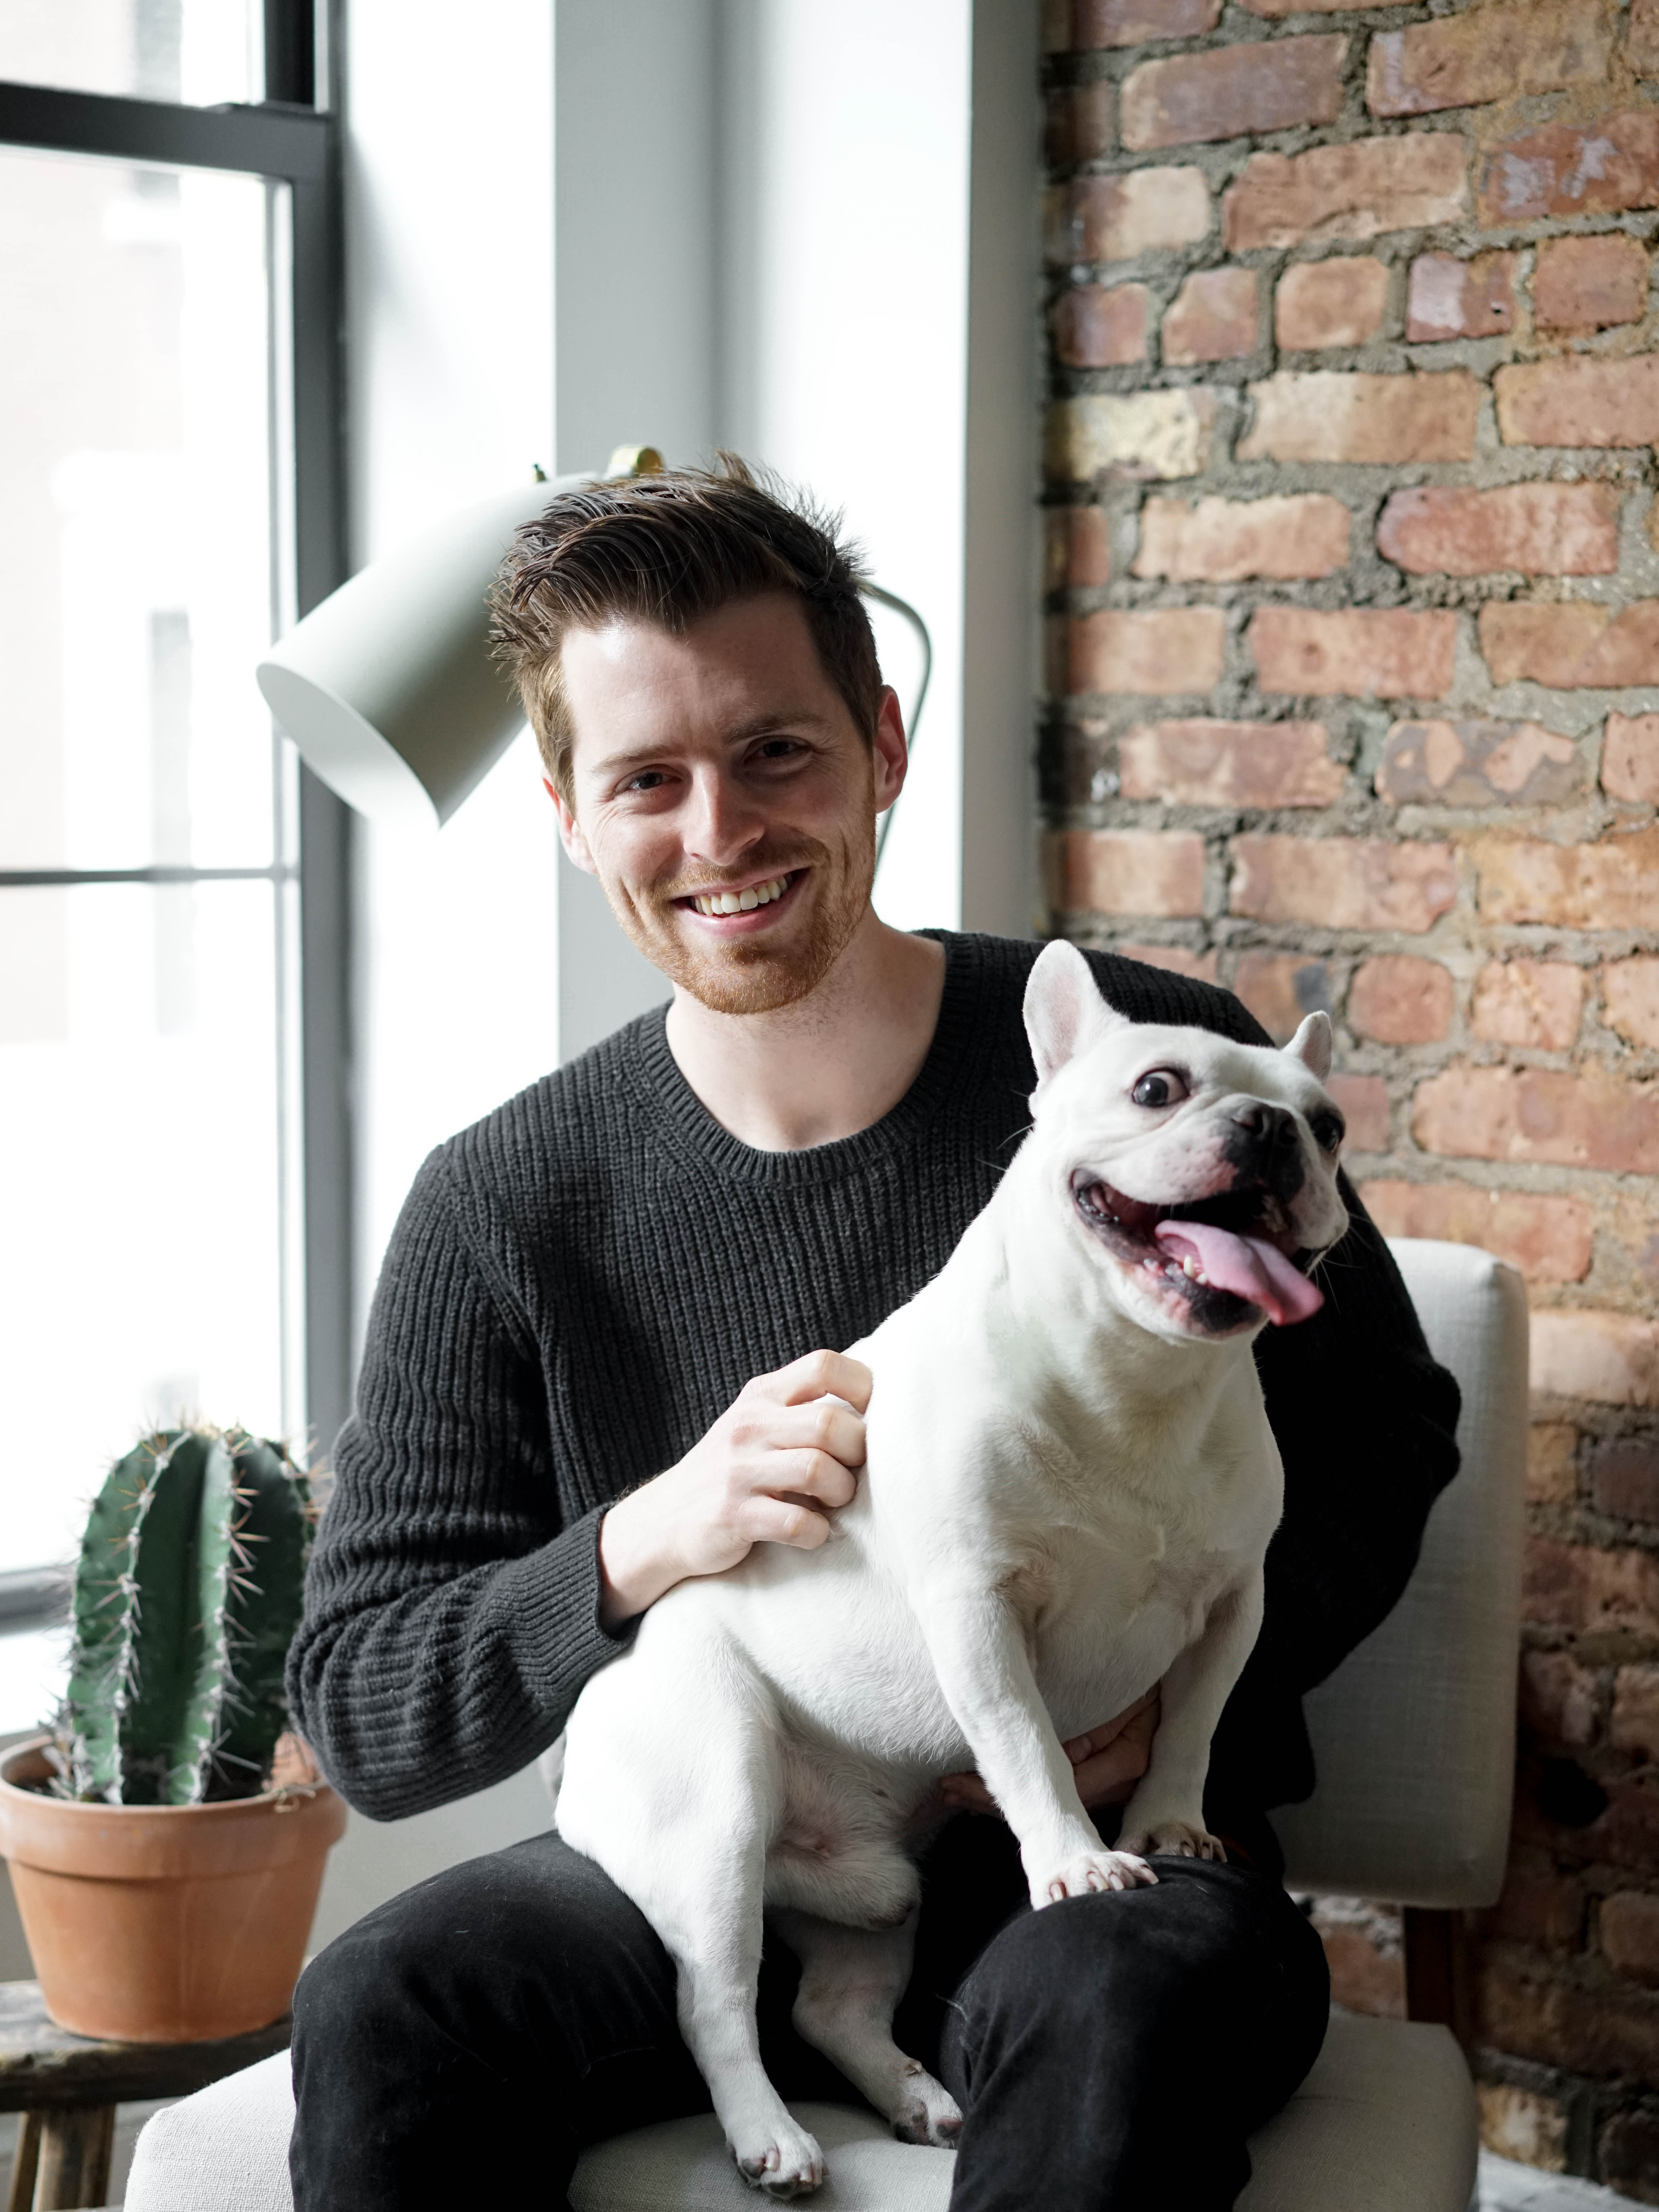
\includegraphics[scale=0.06]{../joelpics/joel.jpg}   &
  
\includegraphics[scale=0.22]{../joelpics/IMG_4133.png}
\end{tabular}
\end{centering}
\end{frame}

\begin{frame}\frametitle{What is context of our work?}
\begin{enumerate}[(i)]
  \item Our work is motivated by the need to design database and software systems
  that support modeling ownership and authorization correctly.
  \item This could be called ``Blockchain for finance/enterprise\ldots done right''
  \item And our particular approach is around developing a functional model
  of linear logic, applying the compiler engineering knowledge ghc and related
  systems embody, and our work is about building a programming language
  that prevents errors in ownership descriptions.
\end{enumerate}

\end{frame}

\begin{frame}\frametitle{What we're here to share today}
  \begin{enumerate}[(i)]
    \item Motivate linearity/ownership with some simple but nontrivial examples of ownership modeled
    in Haskell. We only need the idea of a linear pair for this.
    \item Show how catchable pure exceptions break type safety/soundness of linearity.
    \item Explain the 6 different type formers of classical linear logic in terms of
    their functional haskell analogues.
    \item Show how some of these type formers tie into current work and design directions
    of ghc!
  \end{enumerate}
\end{frame}


% \begin{frame}[t]\frametitle{title}



% \end{frame}

% what is linear logic (high level)

% heres an example (cake or gum)

% linear logic for  haskellers

% how linear logic ideas intersect with design activity in ghc / ghc core




\begin{frame}[fragile]
\frametitle{Whats a Loan?}
\begin{minted}{haskell}


import Control.STM.TQueue
import Control.STM.TVar
newtype InQueue a = IQ (TQueue a)
newtype OutQueue a = OQ  (TQueue a)
data OfferLoan a =  OLoan
  {principal :: Chocolate
  ,repay :: TQueue  BubbleGum }
   --- this is the input side of the queue

-- chocolate for gum later
data Debt where
  Debt :: TQueue BubbleGum -> Debt
takeLoan :: String ->  -- name of loan
    TVar (Map String Debt) -> -- my wallet!
    OfferLoan Candy ->  -- a loan
    STM (Either (OfferLoan Candy) ())
    -- left reject, right accept
\end{minted}
\end{frame}

% measured monoids sound nice for aggregating payments
% integer vs fractional fungibible

\begin{frame}
  \frametitle{What can I do with my bubble gum OutQueue's?}
Alice and Bob both owe me some bubblegum. Rick (who's very risk averse) will happily pay me
for the first 10 pieces of gum I receive, and his friend Morty (always taking risks) will
also pay me for any gum after the first 10! In some circles, this sort of rearrangement
is called a \emph{Sequential Tranche}. Sounds like a great job for Concurrency!


So lets figure out how to recompose the OutQueues from Alice and Bob into new
OutQueues which Rick and Morty can pay me for.

\end{frame}

\begin{frame}[fragile]\frametitle{Concurrency Composes ownership}
\begin{minted}{haskell}
tranche :: OQ BubbleGumm -> OQ BubbleGum
          -> IO (OQ BubbleGum, OQ BubbleGum)
tranche oq1 oq2 = do
    (iqA,oqA) <- makeQueueIO
    (iqB,oqB) <- makeQueueIO
    let doit :: Int -> IO ()
        doit ct iqA iqB = ..
        ... next slide
    _ <- forkIO (doit 0)
    return ()
\end{minted}
\end{frame}

\begin{frame}[fragile]\frametitle{composing continued}
    \begin{minted}{haskell}
doit :: Int -> IO ()
doit ct  = do
  howMuch <- atomically (
  do ma <- tryTake oq1
     mb <- tryTake oq2
     case (ma,mb) of
        (Nothing,Nothing) -> retry
        --  sleep till new stuff
        (Just ra, Nothing) -> do
          if ct > 10
            then putQ oqB ra >> return 1
            else putQ oqA ra >> return 1
        (Nothing,Just ra) ->  ...
        (Just ra,Just rb) ->
          if ct <= 8 then  ...
          else if ct == 9  then ..
          else if ct >= 10 then .. )

    \end{minted}


\end{frame}

% \begin{frame}
%   \frametitle{Motivation}
%   Example of bad core
% \end{frame}

\begin{frame}[fragile]
Consider this innocent program, \ldots are we cartesian closed or merely (symmetric) braided monoidal?
% this should be 2-3 slides in after 1-2 terms/ideas some intro stuff
% \begin{onlyenv}<1>
\begin{minted}{haskell}
module BadUncurry where
import Control.Exception

data Fst a = Only a deriving (Show, Typeable, Exception)

badFst :: (Typeable a, Show a) => a -> b -> a
badFst a = throw (Only a)

notOnly (Only a) = a

nonLinear :: (Show a, Typeable a) => (a, b) -> IO a
nonLinear pr = catch
  (return  (uncurry badFst pr))
  (return . notOnly)
\end{minted}
\end{frame}


% \begin{frame}[fragile]
% what next? What if we replaced our definition of uncurry?
% \begin{minted}{haskell}
% linearUncurry :: (a,b) -> ((# a , b #) -> c) -> c
% \end{minted}
% this version of uncurry doesn't allow an exceptional definition of first!
% \end{frame}

% \begin{frame}
%   \frametitle{Demand Analysis}
%   What's the relationship to demand analysis?

%   GHC ALREADY has a very precise sort of linear logic, ... usage annotations
% \end{frame}

% \begin{frame}
%   \frametitle{Demand Analysis}
%   Demand analysis has more possible demands:

%   {\large Strictness demands}
%   \begin{itemize}
%     \item B: hyperstrict
%     \item L: lazy
%     \item S: head strict
%     \item S(s1 ... sn): structured product demand
%     \item C(s): call demand
%   \end{itemize}

%   {\large Absence / usage demands}
%   \begin{itemize}
%     \item A: unused
%     \item U: used on some execution path
%     \item H: head-used (value used but components are ignored)
%     \item U(u1 ... un): structured usage demand
%     \item C(u): call-demand
%   \end{itemize}
% \end{frame}

% \begin{frame}
%   \frametitle{Demand Analysis}
%   We end up with demands like \tt{<S,U><S,U(UA)>m}.
% \end{frame}

% \begin{frame}
%   \frametitle{Demand Analysis}
%   But the details aren't important
% \end{frame}

% \begin{frame}
%   \frametitle{Demand Analysis}
%   Perhaps the main difference is that demand analysis is focused on \emph{inferring} usage without annotations, while a linear core would have checked annotations.
% \end{frame}

\end{document}
